\section{External Interface Requirements}

\subsection{User Interfaces}
\begin{figure}[H]
      \centering
      
\includegraphics[width=\textwidth]{RASD/Assets/User interfaces/login.png}
      \caption{Login page}
      \label{fig:Login page}
\end{figure}
\begin{figure}[H]
      \centering
      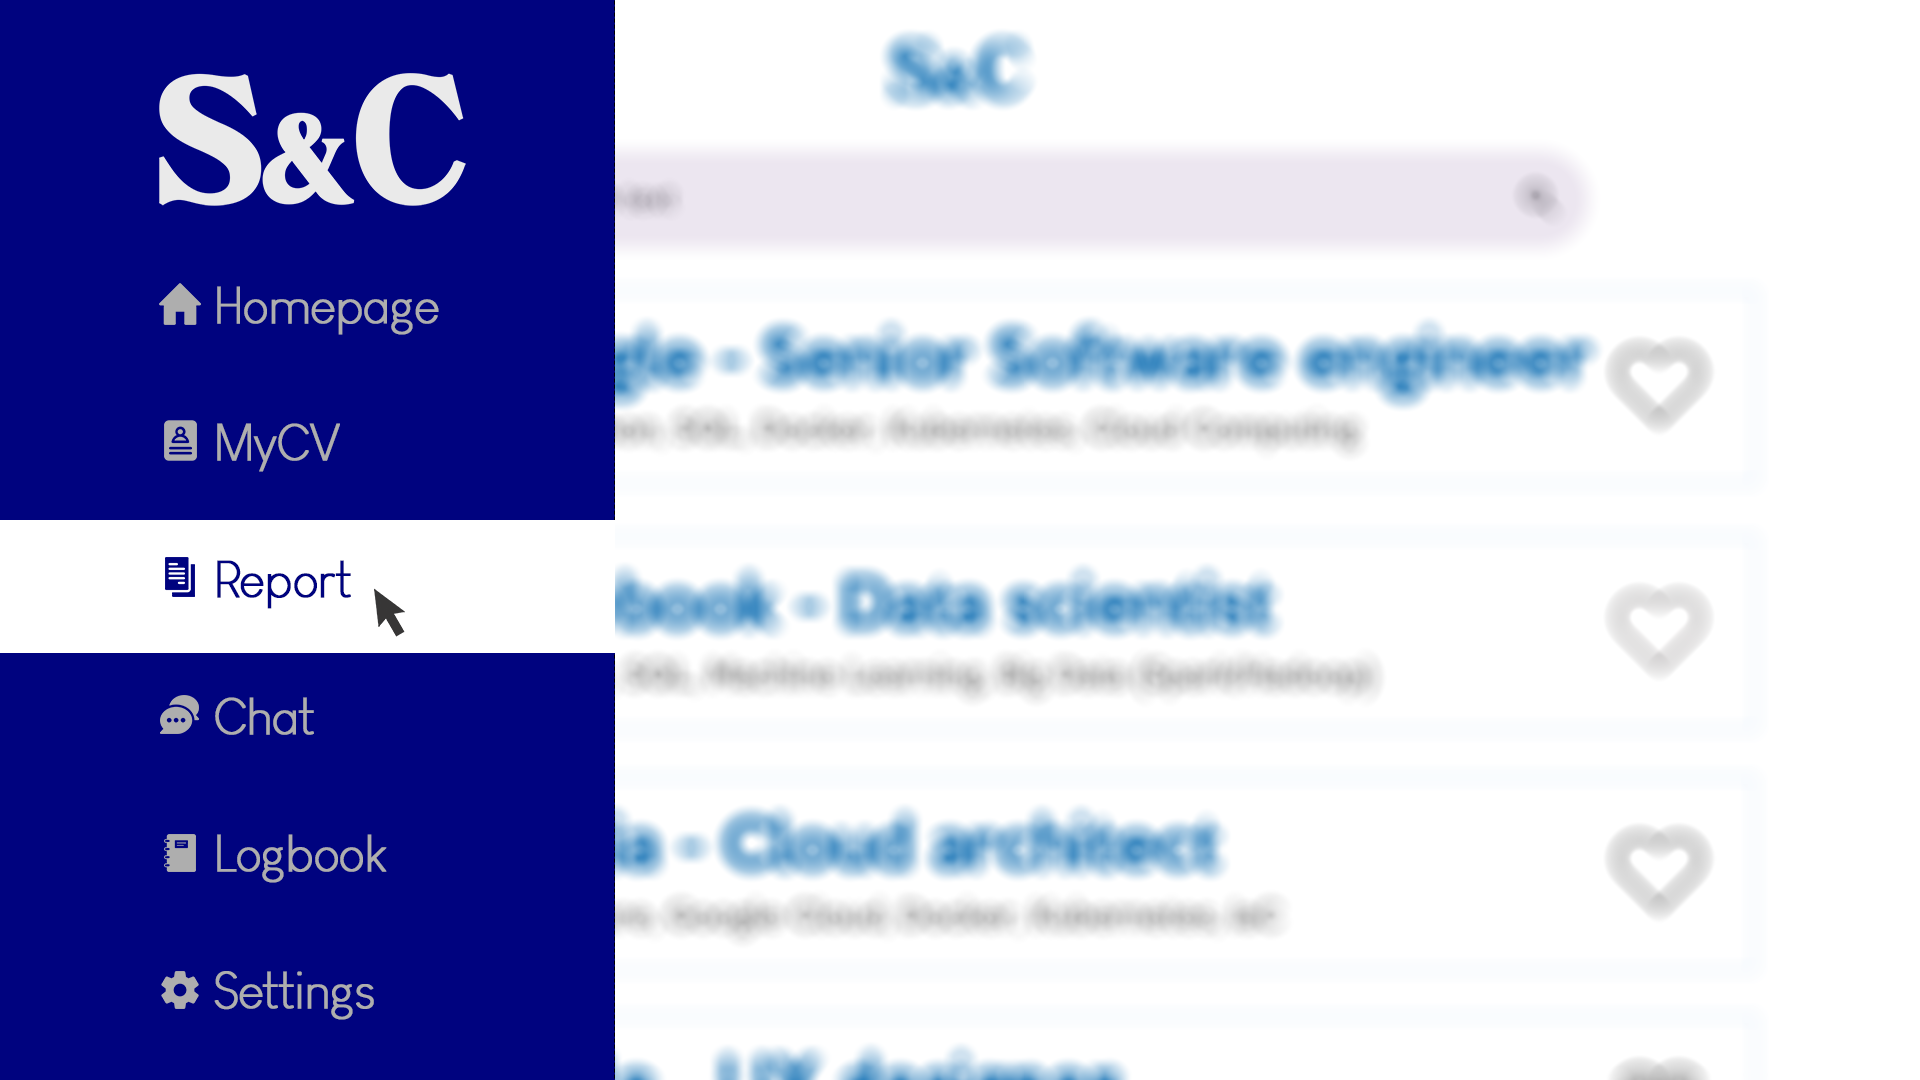
\includegraphics[width=\textwidth]{RASD/Assets/User interfaces/sidebar.png}
      \caption{Student Sidebar}
      \label{fig:Student Sidebar}
\end{figure}
\begin{figure}[H]
      \centering
      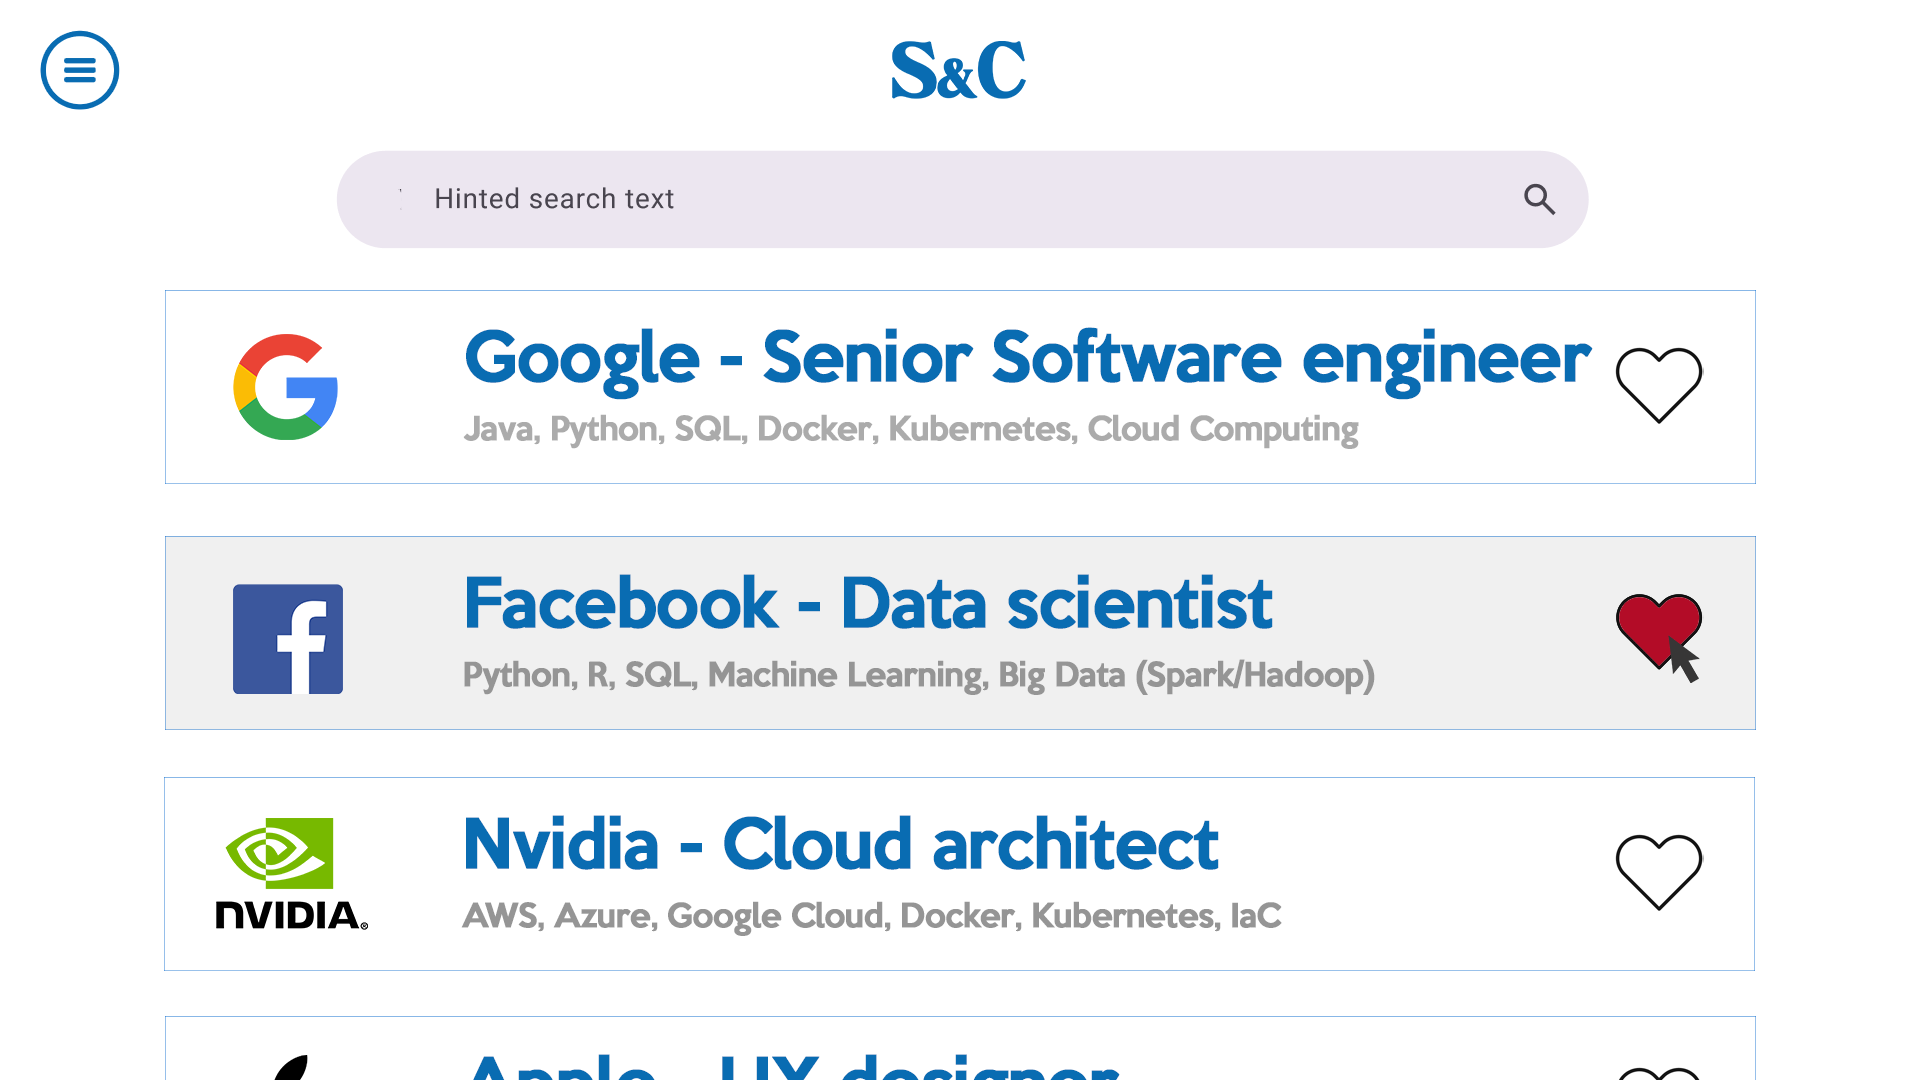
\includegraphics[width=\textwidth]{RASD/Assets/User interfaces/Homepage_student.png}
      \caption{HomePage Student}
      \label{fig:HomePage Student}
\end{figure}
\begin{figure}[H]
      \centering
      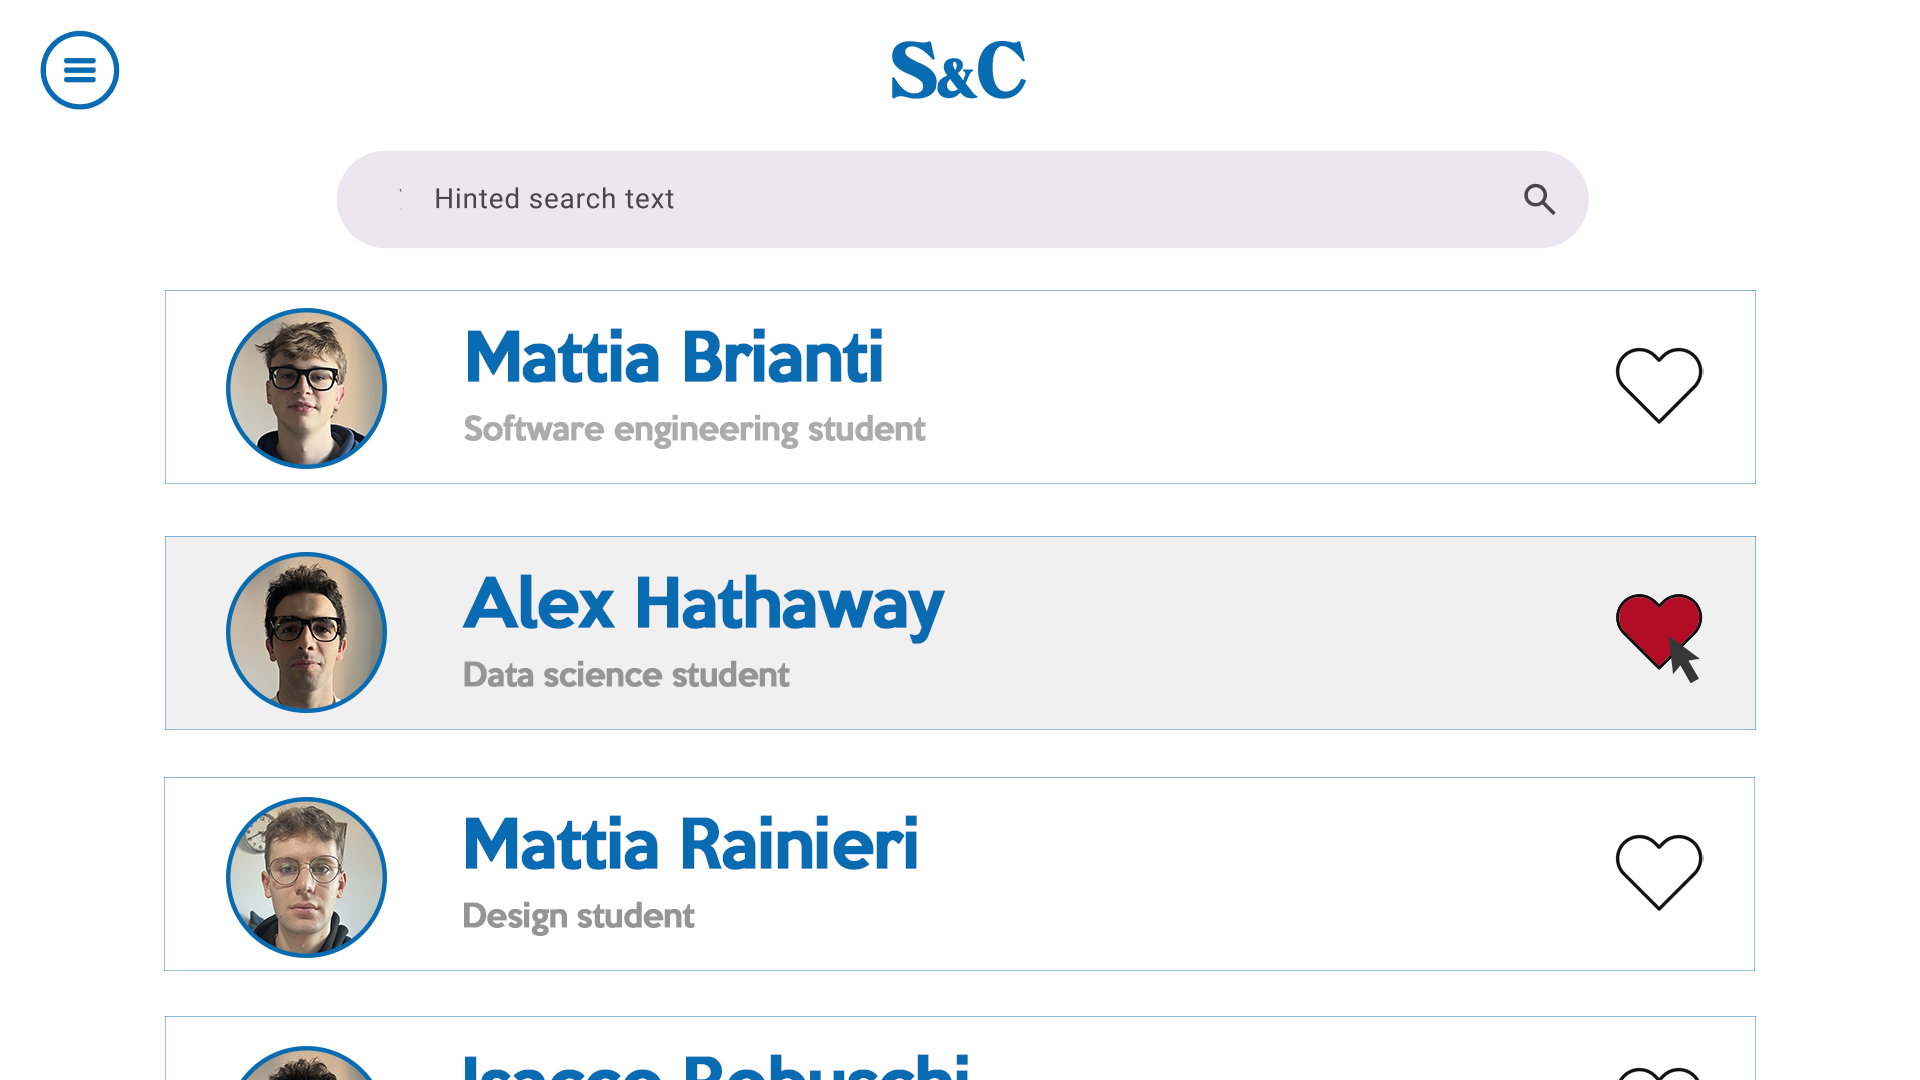
\includegraphics[width=\textwidth]{RASD/Assets/User interfaces/Homepage Company.png}
      \caption{HomePage Company}
      \label{fig:HomePage Company}
\end{figure}


\subsection{Hardware Interfaces}
The system does not need any specific hardware, each user will need a browser with an Internet connection in order to communicate with the platform's servers.

\subsection{Software Interfaces}
\begin{enumerate}
    \item \textbf{Videocall meeting}
    \item \textbf{AI tool for matchmaking}
    \item \textbf{Databases Interface}
\end{enumerate}

\subsection{Comunication Interfaces}
\begin{enumerate}
    \item \textbf{eduGAIN Radius} - in order to allow a native single sign-on for all European universities. \cite{eduGAIN}
    \item \textbf{OAuth2} - is a very commonly used standard in the enterprise environment, to consent the adoption of Single Sign On (SSO) with external platform.
    \item \textbf{HyperText Transfer Protocol over Secure Socket Layer (HTTPS)} - used for all communications between client  and server.
    \item \textbf{Simple Mail Transfer Protocol (SMTP)} - , a standard protocol for email transmission, which is used by this platform to send notifications through email.
\end{enumerate}

\section{Functional Requirements}
\begin{enumerate}[label=\textbf{R\arabic*}:,ref=R\arabic*,leftmargin=1.3cm]
    \labelleditem{The system shall allow users to log in with SSO.}
    \labelleditem{The system shall allow the student to provide information for their CVs.}
        \begin{enumerate}[label=\textbf{R\arabic{enumi}.\arabic*}:,ref=R\arabic{enumi}.\arabic*, leftmargin=*]
            \labelledsubitem{The system shall allow the students to specify their personal information, like name, contact and personal ambition.}
            \labelledsubitem{The system shall allow the students to specify their education experience, including their academic background.}
            \labelledsubitem{The system shall allow the students to specify their past work experience, specifying job title, company name, duration and technologies used.}
            \labelledsubitem{The system will allow students to specify their technical and soft skills.}
            \labelledsubitem{The system shall allow the students to specify their project and research, including the title, duration and description}
            \labelledsubitem{The system shall allow the students to specify their extracurricular activities, including the name, organization and achievements.}
            \labelledsubitem{The system will allow students to specify their knowledge of languages, including the level and any certifications.}
            \labelledsubitem{The system shall allow students to specify their availability.}
            \labelledsubitem{The system will allow the students to add additional information.}
        \end{enumerate}
    \labelleditem{The system shall allow the students to join an internship.}
        \begin{enumerate}[label=\textbf{R\arabic{enumi}.\arabic*}:,ref=R\arabic{enumi}.\arabic*, leftmargin=*]
            \labelledsubitem{The system shall help the students to create a customized CV for each company.}
        \end{enumerate}
   \labelleditem{The system shall allow the students to be notified when a new applicable internship becomes available.}
    \labelleditem{The system shall allow the company employee to create an internship.}
        \begin{enumerate}[label=\textbf{R\arabic{enumi}.\arabic*}:,ref=R\arabic{enumi}.\arabic*, leftmargin=*]
            \labelledsubitem{The system shall allow the company employee to specify the title of the internship.}
            \labelledsubitem{The system shall allow the company employee to specify the description, helped by an AI, of the internship.}
            \labelledsubitem{The system shall allow the company employee to specify the requirement of the internship.}
            \labelledsubitem{The system shall allow the company employee to specify the duration of the internship.}
            \labelledsubitem{The system shall allow the company employee to specify the availability of the internship.}
            \labelledsubitem{The system shall allow the company employee to specify other information about the internship.}
        \end{enumerate}
    \labelleditem{The system shall allow the company employee to be notified when a new potentially interesting student becomes available.}
    \labelleditem{The system shall allow the student to view a personalized homepage after inserting his CV's information.}
    \labelleditem{The system shall allow the company employee to view a personalized homepage after publishing an internship.}
    \labelleditem{The system shall allow the company to write a complaint to the university.}
    \labelleditem{The system shall allow the students to write a complaint to the university.}
    \labelleditem{The system shall allow students to chat with his company.}
    \labelleditem{The system shall allow companies employee to chat with his trainee.}
    \labelleditem{The system shall allow universities employee to chat with his students.}
    \labelleditem{The system shall allow the student to insert initial information.}
    \labelleditem{The system shall allow the student and the company to arrange a meeting.}
    \labelleditem{The system shall send a meeting link for the interview to the student and the company.}
    \labelleditem{The system shall allow the student to write on a logbook to inform the university on the status of his internship.}
\end{enumerate}

\subsection{Use case diagrams}
    \subsubsection{Student}

    \begin{figure}[H]
        \centering
        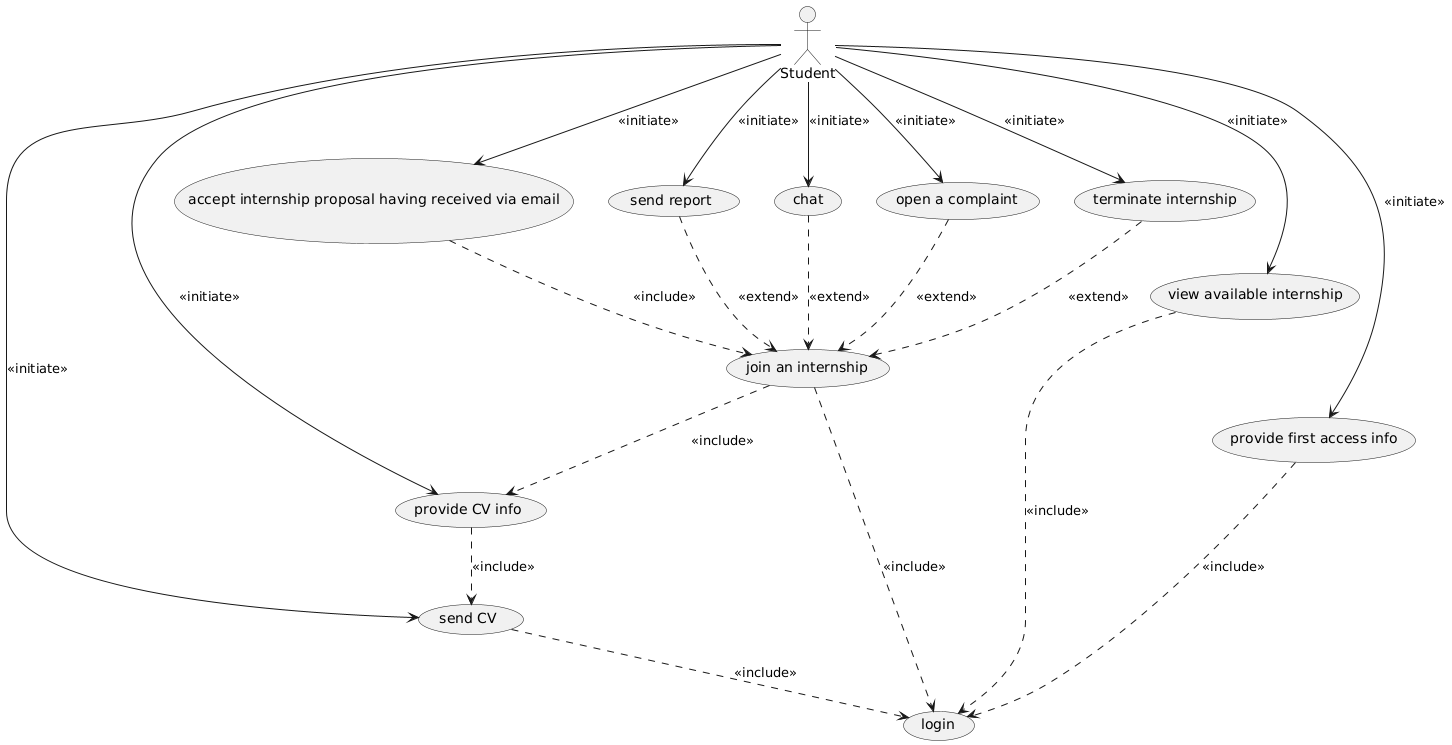
\includegraphics[width=0.8\textwidth]{RASD/Assets/UseCaseDiagram/student.png}
        \caption{Student's use case diagram.}
        \label{fig:Student's use case diagram}
    \end{figure}

\subsubsection{Company employee}

    \begin{figure}[H]
        \centering
        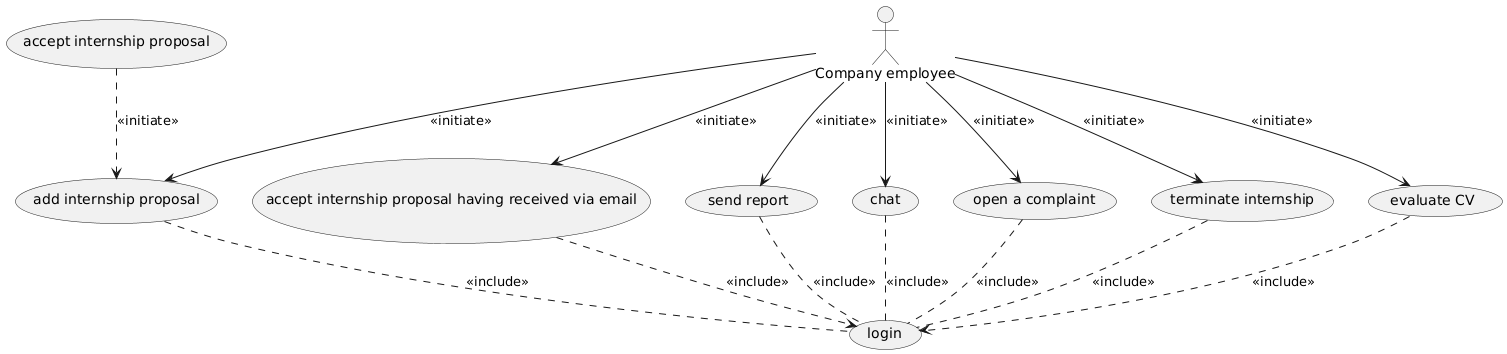
\includegraphics[width=0.8\textwidth]{RASD/Assets/UseCaseDiagram/company.png}
        \caption{Company employee's use case diagram.}
        \label{fig:Company employee's use case diagram}
    \end{figure}

\subsubsection{University employee}

    \begin{figure}[H]
        \centering
        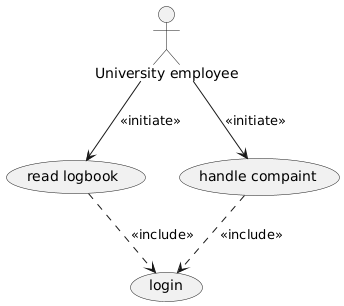
\includegraphics[width=0.8\textwidth]{RASD/Assets/UseCaseDiagram/university.png}
        \caption{University employee's use case diagram.}
        \label{fig:University employee's use case diagram}
    \end{figure}

\pagebreak
\subsection{Use cases}

    \textbf{UC1}
    \nopagebreak
    \begin{table}[H]
    \centering
    \begin{tabular}{|l|p{11.9cm}|}
        \hline
        \textbf{Name}            & Student's first platform access                     \\\hline
        \textbf{Actor}           & Student         \\\hline
        \textbf{Entry condition} &
        \begin{itemize}
              \item Student has never accessed the platform
        \end{itemize}                                        \\\hline
        \textbf{Event flow}      &
        \begin{enumerate}[label=\arabic*.]
              \item The student, who has an internet connection, inserts the URL in the browser.
              \item The student clicks on the login button.
              \item The student inserts his email and will be redirected to the university SSO.
              \item The students selects his academic interests.
        \end{enumerate}            \\\hline
        \textbf{Exit condition}  & The student is redirected to the homepage\\\hline
        \textbf{Exception}       &  Student's credentials are not valid. In this case a pop up will be shown with a message to that effect.   \\\hline
    \end{tabular}
    \caption{Student's first platform access}
    \label{table:Student's first platform access}
    \end{table}

    \begin{figure}[H]
        \centering
        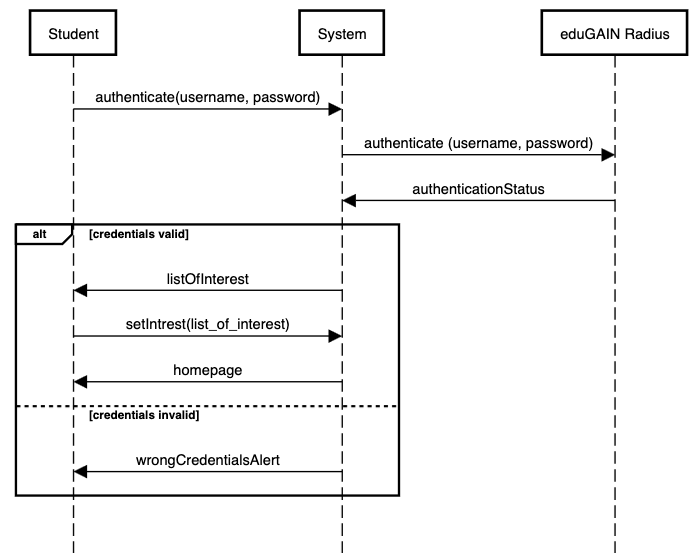
\includegraphics[width=0.8\textwidth]{Assets/SequenceDiagrams/1-login.png}
        \caption{Student's first platform access.}
        \label{fig:Student's first platform access}
    \end{figure}


    \textbf{UC2}
    \nopagebreak
    \begin{table}[H]
    \centering
    \begin{tabular}{|l|p{11.9cm}|}
        \hline
        \textbf{Name}            & Student inserts his CV information in the InitialForm
        \\\hline
        \textbf{Actor}           & Student         \\\hline
        \textbf{Entry condition} &
        \begin{itemize}
              \item Student is already logged in
              \item Student has never provided his information in "My CV" section
        \end{itemize}                                        \\\hline
        \textbf{Event flow}      &
        \begin{enumerate}[label=\arabic*.]
            \item The student press on the contact button.
            \item The student, altered by a pop-up, follows the redirect to the "My CV" page.
            \item The student fills out the form.
            \item The student click on the save button.
        \end{enumerate}            \\\hline
        \textbf{Exit condition}  & The system will show a message confirming the success of the operation.\\\hline
        
        \textbf{Exception}       &  Student misses to compile some fields. In this case, an alert pop-up is shown.  \\\hline
    \end{tabular}
    \caption{Student provides his CV’s information to the platform.}
    \label{table:Student provides his CV’s information to the platform}
    \end{table}

    \begin{figure}[H]
        \centering
        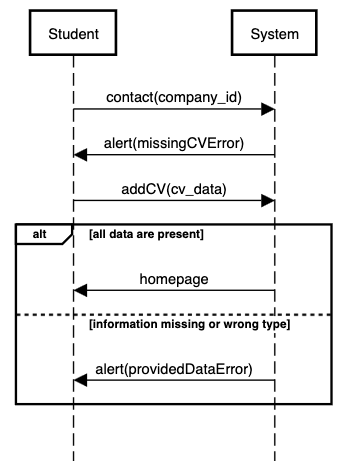
\includegraphics[width=0.8\textwidth]{RASD/Assets/SequenceDiagrams/2-student-provide-his-cv.png}
        \caption{Student inserts information from their CV in the platform.}
        \label{fig:Student provides his CV’s information to the platform}
    \end{figure}


    \textbf{UC3}
    \nopagebreak
    \begin{table}[H]
    \centering
    \begin{tabular}{|l|p{11.9cm}|}
        \hline
        \textbf{Name}            & Student search and contact the company \\\hline
        \textbf{Actor}           & Student, Company Employee         \\\hline
        \textbf{Entry condition} &
        \begin{itemize}
              \item Student is already logged in
              \item Student has already compiled his Curriculum Vitae
        \end{itemize}                                        \\\hline
        \textbf{Event flow}      &
        \begin{enumerate}[label=\arabic*.]
              \item The student opens the homepage.
              \item The student clicks on contact button next to the interested company.
              \item The platform generates a customized CV.
              \item The student reads the proposal customized and send it.
              \item The company receives the customized CV.
        \end{enumerate}            \\\hline
        \textbf{Exit condition}  & The company employee approves the student's CV.\\\hline
        \textbf{Exception}       &  
        \begin{itemize}
              \item The student does not approve the customized CV proposed by the platform. In this case, the student manually modifies it.
              \item The company employee does not approve the student's CV. In this case, the employee can reject the proposal.  
        \end{itemize} 
        \\\hline
    \end{tabular}
    \caption{Student finds the company and contacts it via the platform}
    \label{table:Student search and contact the company}
    \end{table}

    \begin{figure}[H]
        \centering
        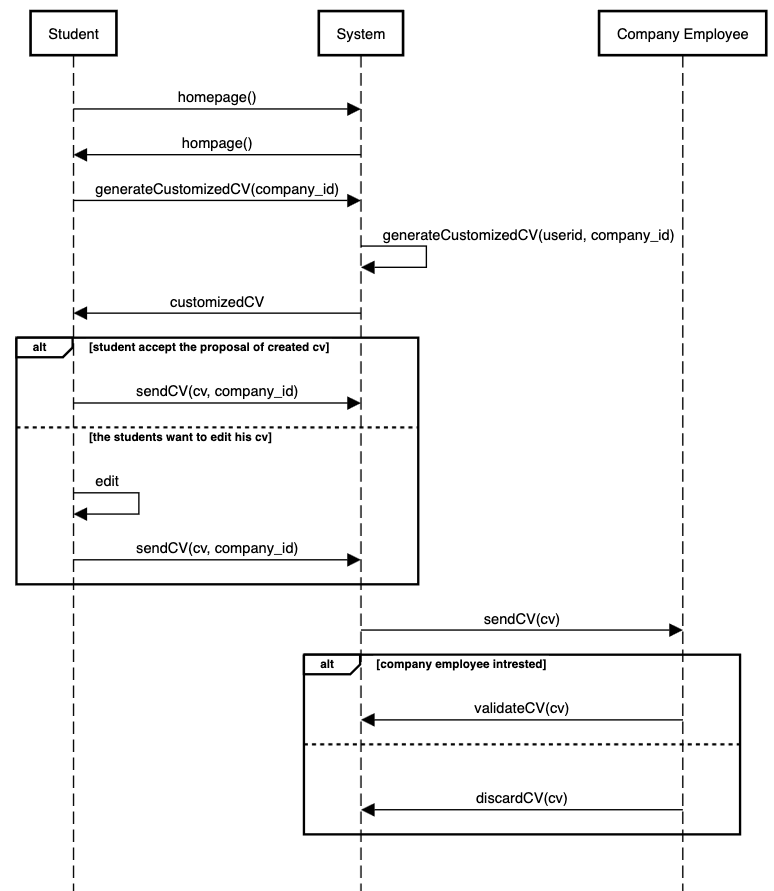
\includegraphics[width=0.8\textwidth]{RASD/Assets/SequenceDiagrams/3-student-contact-company.png}
        \caption{Student finds the company and contacts it via the platform.}
        \label{fig:Student search and contact the company}
    \end{figure}
    

    \textbf{UC4}
    \nopagebreak
    \begin{table}[H]
    \centering
    \begin{tabular}{|l|p{11.9cm}|}
        \hline
        \textbf{Name}            & A company publishes an advertisement about the internships they are
offering \\\hline
        \textbf{Actor}           & Company Employee, Student possibly interested on that opportunity.        \\\hline
        \textbf{Entry condition} &
        \begin{itemize}
              \item Company was already approved on the platform
        \end{itemize}                                        \\\hline
        \textbf{Event flow}      &
        \begin{enumerate}[label=\arabic*.]
              \item The company employee logs in using his company's credentials.
              \item The company employee opens the "Create Job Opportunity" page.
              \item The company employee inserts all the information requested into the platform.
              \item A successful message is shown, and, after a couple of seconds, the company employee is redirected to the homepage.
        \end{enumerate}            \\\hline
        \textbf{Exit condition}  & Interested students receive a notification \\\hline
        \textbf{Exception}       &  Company employee has not completed all fields in the form. In this case, an alert message is shown.   \\\hline
    \end{tabular}
    \caption{Student search and contact the company}
    \label{table:Student search and contact the company}
    \end{table}

    \begin{figure}[H]
        \centering
        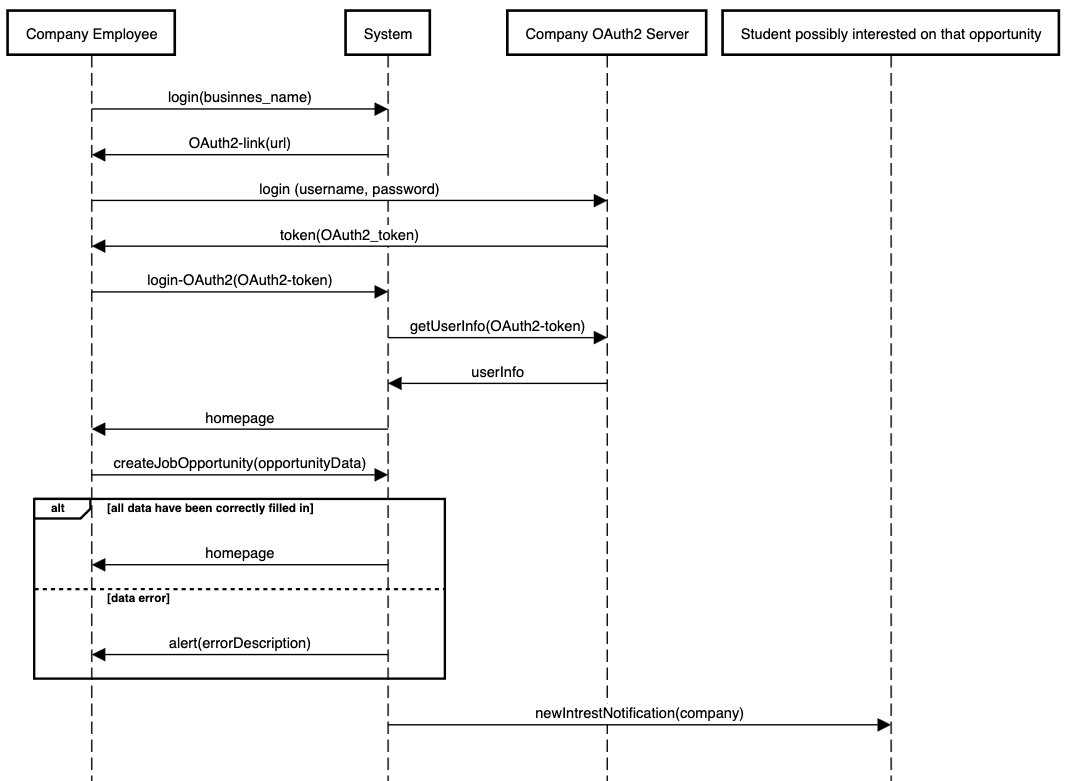
\includegraphics[width=0.8\textwidth]{RASD/Assets/SequenceDiagrams/4-company-publish-and-adv.png}
        \caption{Student finds the company and contacts it via the platform.}
        \label{fig:Student search and contact the company}
    \end{figure}


    \textbf{UC5}
    \nopagebreak
    \begin{table}[H]
    \centering
    \begin{tabular}{|l|p{11.9cm}|}
        \hline
        \textbf{Name}            & Student search through the internships and contact the company \\\hline
        \textbf{Actor}           & Student, Company Employee         \\\hline
        \textbf{Entry condition} &
        \begin{itemize}
              \item Student is already logged in
              \item Student has already compiled his Curriculum Vitae
              \item A Company has published an internship that may interest the student.
        \end{itemize}                                        \\\hline
        \textbf{Event flow}      &
        \begin{enumerate}[label=\arabic*.]
              \item The student receive an email.
              \item The student click on the link contained in the email.
              \item The student is interested on that specific internship, so he presses the "Contact" button.
              \item The student approves the custom generated CV.
        \end{enumerate}            \\\hline
        \textbf{Exit condition}  & Student clicks the "Send" button.\\\hline
        \textbf{Exception}       &  
        \begin{itemize}
            \item The student is not interested in the proposed internship. In this case, the student simply ignores the notification.
            \item The student does not approve the customized CV proposed by the platform. In this case, the student must manually modify it.
        \end{itemize} 
        \\\hline
    \end{tabular}
    \caption{Student searches through available internships and contacts the company}
    \label{table:Student search through the internhisps and contact the company}
    \end{table}
oi
    \begin{figure}[H]
        \centering
        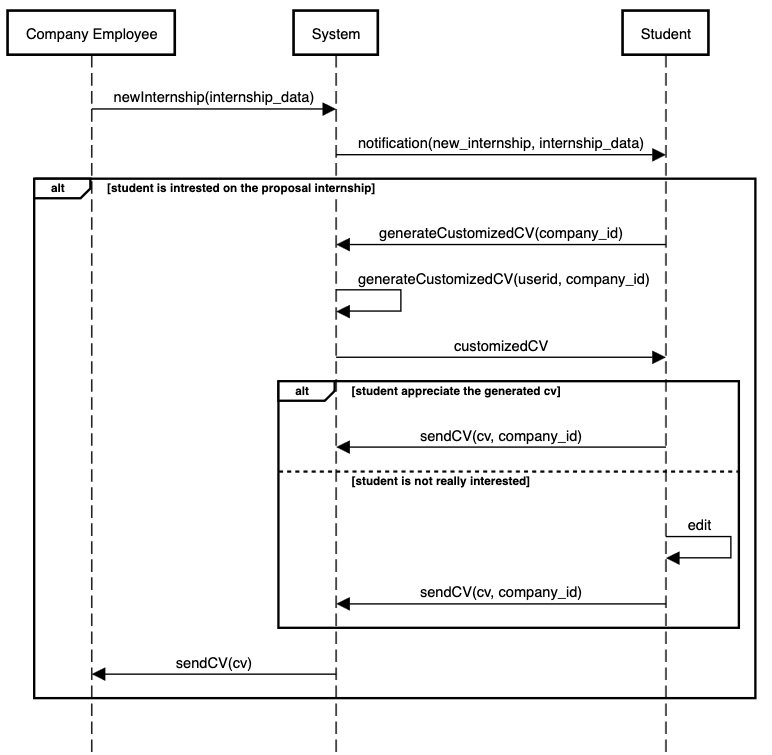
\includegraphics[width=0.8\textwidth]{RASD/Assets/SequenceDiagrams/5-student-receives-a-notification.png}
        \caption{Student receives a notification about the availability of an internship that might interest him.}
        \label{fig:Student receive a notification about the availability of an internship that might interest him}
    \end{figure}

    \textbf{UC6}
    \nopagebreak
    \begin{table}[H]
        \centering
        \begin{tabular}{|l|p{11.9cm}|}
        \hline
        \textbf{Name}            & A company receives a notification about the availability of a student CV corresponding to their needs \\\hline
        \textbf{Actor}           & Student, Company Employee       \\\hline
        \textbf{Entry condition} &
        \begin{itemize}
              \item Students has just completed his "My CV" section
        \end{itemize}                                        \\\hline
        \textbf{Event flow}      &
        \begin{enumerate}[label=\arabic*.]
              \item The system will start a matchmaking process between the student and opened internship positions.
              \item The system sends a notification to all of the company employees who may be interested in the new student.
              \item The company employee, who receives the notification, clicks on the "View Profile" button to obtain more detailed information about his CV.
              \item The company employee clicks on send message, near the student name, to contact him.
              
        \end{enumerate}            \\\hline
        \textbf{Exit condition}  & The company employee sends a message to the student  \\\hline
        \textbf{Exception}       &  The company employee does not really feel interested in the student's proposal. In this case, he just ignores the mail.   \\\hline
        \end{tabular}
        \caption{A company receive a notification about the availability of a student CV corresponding to their needs.}
        \label{table:A company receive a notification about the availability of a student CV corresponding to their needs}
    \end{table}

    \begin{figure}[H]
        \centering
        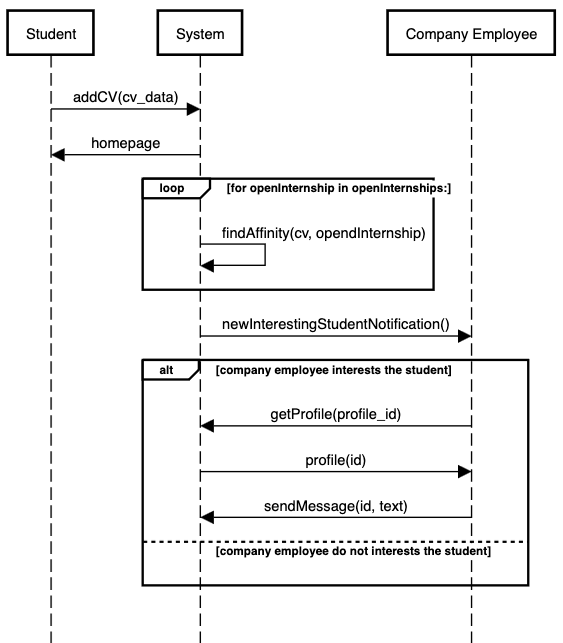
\includegraphics[width=0.8\textwidth]{RASD/Assets/SequenceDiagrams/6-matchmaking-new-student.png}
        \caption{A company receives a notification about the availability of a student CV corresponding to their needs.}
        \label{fig:A company receive a notification about the availability of a student CV corresponding to their needs}
    \end{figure}


    \textbf{UC7}
    \nopagebreak
    \begin{table}[H]
        \centering
        \begin{tabular}{|l|p{11.9cm}|}
        \hline
        \textbf{Name}            & Student gives final feedback about the internship \\\hline
        \textbf{Actor}           & Student     \\\hline
        \textbf{Entry condition} &
        \begin{itemize}
              \item Student has just finished his internship
        \end{itemize}                                        \\\hline
        \textbf{Event flow}      &
        \begin{enumerate}[label=\arabic*.]
              \item The student opens the sidebar and click on "Report" button.
              \item The system recognizes that he has just finished an internship, so shows the "Give us your final feedback" form.
              \item The student fills the form.
              
        \end{enumerate}            \\\hline
        \textbf{Exit condition}  & Click on "Submit" button  \\\hline
        \textbf{Exception}       &  The student does not want to provide his feedback. In this case, no actions are required.   \\\hline
        \end{tabular}
        \caption{Student gives final feedback about the internship.}
        \label{table:Student gives final feedback about the internship}
    \end{table}

    \begin{figure}[H]
        \centering
        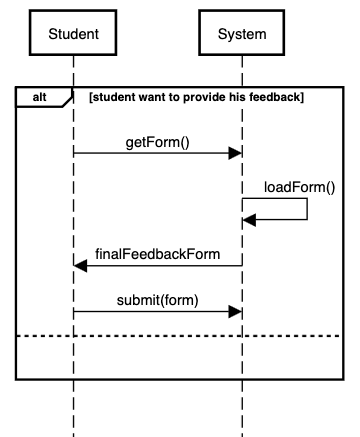
\includegraphics[width=0.8\textwidth]{RASD/Assets/SequenceDiagrams/7-internship-final-form.png}
        \caption{Student gives final feedback about the internship.}
        \label{fig:Student gives final feedback about the internship}
    \end{figure}


    \textbf{UC8}
    \nopagebreak
    \begin{table}[H]
        \centering
        \begin{tabular}{|l|p{11.9cm}|}
        \hline
        \textbf{Name}            & The University receive the request to end an internship from a student and contacts the company to end it \\\hline
        \textbf{Actor}           & University employee     \\\hline
        \textbf{Entry condition} &
        \begin{itemize}
              \item University employee receives an email 
        \end{itemize}                                        \\\hline
        \textbf{Event flow}      &
        \begin{enumerate}[label=\arabic*.]
              \item The university employee clicks on the "See complaint" button in the email, so a new page is opened.
              \item The university employee opens the student's profile by clicking on his name.
              \item The university employee clicks on "Terminate Internship" button.
              
        \end{enumerate}            \\\hline
        \textbf{Exit condition}  & The university employee confirms the pop-up.  \\\hline
        \textbf{Exception}       &    \\\hline
        \end{tabular}
        \caption{University receive the request of ending an internship from a student and contacts the company to end it .}
        \label{table:University receive the request of ending an internship from a student and contact the company to end it }
    \end{table}

    \begin{figure}[H]
        \centering
        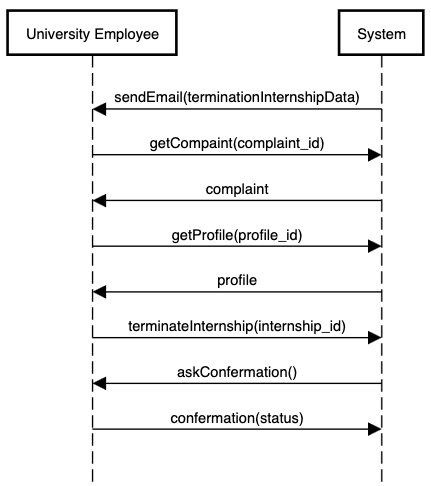
\includegraphics[width=0.8\textwidth]{RASD/Assets/SequenceDiagrams/8-student-end-internship.png}
        \caption{University receive the request of ending an internship from a student and contacts the company to end it .}
        \label{fig:University receive the request of ending an internship from a student and contact the company to end it }
    \end{figure}


    \textbf{UC9}
    \nopagebreak
    \begin{table}[H]
        \centering
        \begin{tabular}{|l|p{11.9cm}|}
        \hline
        \textbf{Name}            & Student complains with the university on the "Report Area" about his ongoing internship \\\hline
        \textbf{Actor}           & Student    \\\hline
        \textbf{Entry condition} &
        \begin{itemize}
              \item The student is not satisfied with his internship
        \end{itemize}                                        \\\hline
        \textbf{Event flow}      &
        \begin{enumerate}[label=\arabic*.]
              \item The students open the S\&C portal and opens the "Report Area" page.
              \item The student completes the form.
        \end{enumerate}            \\\hline
        \textbf{Exit condition}  & Click on "Submit" button  \\\hline
        \textbf{Exception}       &  The student wants re-try to communicate with his company. In this case, the student will send a message through the chat.   \\\hline
        \end{tabular}
        \caption{Student complains with the university on the "Report Area" about his ongoing internship.}
        \label{table:Student complains with the university on the "Report Area" about his ongoing internship}
    \end{table}

    \begin{figure}[H]
        \centering
        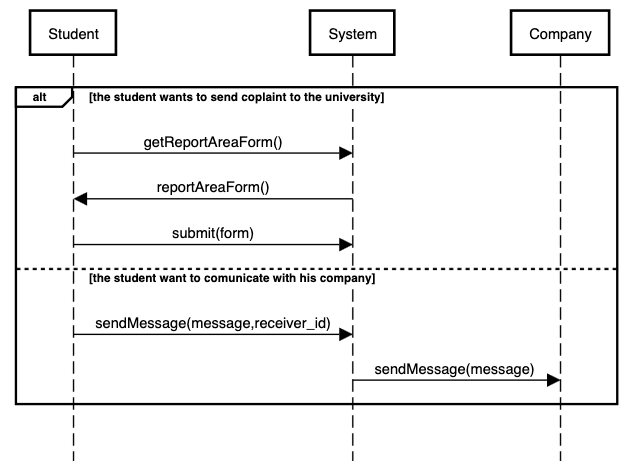
\includegraphics[width=0.8\textwidth]{RASD/Assets/SequenceDiagrams/9-student-sends-a-complaint.png}
        \caption{Student complains with the university on the "Report Area" about his ongoing internship.}
        \label{fig:Student complains with the university on the "Report Area" about his ongoing internship}
    \end{figure}

    \textbf{UC10}
    \nopagebreak
    \begin{table}[H]
        \centering
        \begin{tabular}{|l|p{11.9cm}|}
        \hline
        \textbf{Name}            & The company complains about the student in the internship \\\hline
        \textbf{Actor}           & Company employee, university employee    \\\hline
        \textbf{Entry condition} &
        \begin{itemize}
              \item The company is not satisfied with the student internship
        \end{itemize}                                        \\\hline
        \textbf{Event flow}      &
        \begin{enumerate}[label=\arabic*.]
              \item The company employee open the S\&C portal and opens the "Report Area" page.
              \item The company employee selects the involved student's name.
              \item The company employee clicks on "Report" button in student's page.
              \item The company employee now can fill out the form, describing the problem details.
              \item The company employee clicks on "Submit" button
        \end{enumerate}            \\\hline
        \textbf{Exit condition}  & The University receives a notification about the report.\\\hline
        \textbf{Exception}       &  Some form values are missing. In this case, an alert pop-up will be shown.\\\hline
        \end{tabular}
        \caption{The company complains about the student taking the internship.}
        \label{table:The company complains about the student taking the internship}
    \end{table}

    \begin{figure}[H]
        \centering
        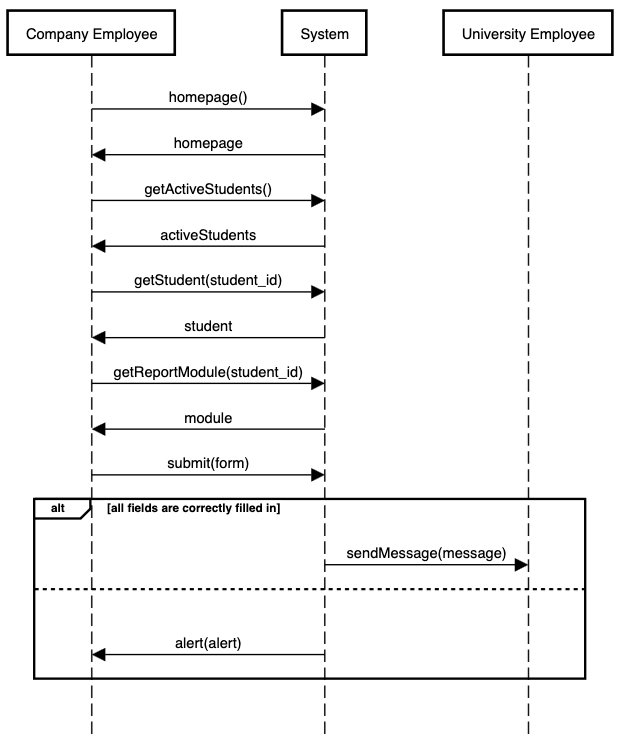
\includegraphics[width=0.8\textwidth]{RASD/Assets/SequenceDiagrams/10-company-sends-a-complaint.png}
        \caption{The company complains about the student taking the internship.}
        \label{fig:The company complains about the student taking the internship}
    \end{figure}

\subsection{Requirements mapping}
This section shows how the $R\land D \models G$ holds.
In particular, the following traceability matrix associates domain assumptions and requirements to goals.
After that, to facilitate reading, the text of all the assumptions and all the requirements related to each goal is reported.
\begin{table}[H]
      %\caption*{\textbf{Title}}
      \centering
      \begin{tabular}{|l|p{8cm}|p{5cm}|}
            \hline
            \textbf{Goal ID} & \textbf{Requirement ID} & \textbf{Domain assumption ID}      \\\hline
            \ref{{G1}}       & \ref{{R1}}, \ref{{R2}}, \ref{{R2.1}}, \ref{{R2.2}}, \ref{{R2.3}}, \ref{{R2.4}}, \ref{{R2.5}}, \ref{{R2.6}}, \ref{{R2.7}}, \ref{{R2.8}}, \ref{{R2.9}}   & \ref{{D1}}, \ref{{D2}}, \ref{{D3}}                
             \\\hline
             
            \ref{{G2}}       & \ref{{R1}}, \ref{{R5}}, \ref{{R5.1}}, \ref{{R5.2}}, \ref{{R5.3}}, \ref{{R5.4}}, \ref{{R5.5}}, \ref{{R5.6}}
            & \ref{{D1}}, \ref{{D2}}, \ref{{D3}}     \\\hline
            
            \ref{{G3}}
            &
            \ref{{R1}}, \ref{{R5}},\ref{{R5.2}}, \ref{{R5.3}}, \ref{{R5.4}}, \ref{{R5.5}}, \ref{{R5.6}} \ref{{R13}}  
            & 
            \ref{{D1}}, \ref{{D2}}, \ref{{D3}}, \ref{{D6}}, \ref{{D8}}  \\\hline
            
            \ref{{G4}}
            & 
            \ref{{R1}}, \ref{{R4}}, \ref{{R5}}, \ref{{R5.1}}, \ref{{R5.2}}, \ref{{R5.3}}, \ref{{R5.4}}, \ref{{R5.5}}, \ref{{R5.6}}
            & 
            \ref{{D1}}, \ref{{D2}}, \ref{{D3}}, \ref{{D6}}                                \\\hline

            
            \ref{{G5}}       
            &
            \ref{{R1}}, \ref{{R2}}, \ref{{R2.1}}, \ref{{R2.2}}, \ref{{R2.3}}, \ref{{R2.4}}, \ref{{R2.5}}, \ref{{R2.6}}, \ref{{R2.7}}, \ref{{R2.8}}, \ref{{R2.9}}, \ref{{R5}}, \ref{{R5.1}}, \ref{{R5.2}}, \ref{{R5.3}}, \ref{{R5.4}}, \ref{{R5.5}}, \ref{{R5.6}}, \ref{{R6}}
            & 
            \ref{{D1}}, \ref{{D2}}, \ref{{D3}}, \ref{{D6}}                     
            \\\hline
            
            
            \ref{{G6}}
            &
            \ref{{R1}}, \ref{{R2}}, \ref{{R2.1}}, \ref{{R2.2}}, \ref{{R2.3}}, \ref{{R2.4}}, \ref{{R2.5}}, \ref{{R2.6}}, \ref{{R2.7}}, \ref{{R2.8}}, \ref{{R2.9}}, \ref{{R4}}, \ref{{R5}}, \ref{{R5.1}}, \ref{{R5.2}}, \ref{{R5.3}}, \ref{{R5.4}}, \ref{{R5.5}}, \ref{{R5.6}}, \ref{{R6}}, \ref{{R7}}, \ref{{R8}}
            &
            \ref{{D1}}, \ref{{D2}}, \ref{{D3}}, \ref{{D6}}                                \\\hline

            
            \ref{{G7}}
            & 
            \ref{{R1}}, \ref{{R2}}, \ref{{R2.1}}, \ref{{R2.2}}, \ref{{R2.3}}, \ref{{R2.4}}, \ref{{R2.5}}, \ref{{R2.6}}, \ref{{R2.7}}, \ref{{R2.8}}, \ref{{R2.9}}, \ref{{R5}},\ref{{R5.1}}, \ref{{R5.2}}, \ref{{R5.3}}, \ref{{R5.4}}, \ref{{R5.5}}, \ref{{R5.6}}, \ref{{R11}}, \ref{{R12}}
            & 
            \ref{{D1}}, \ref{{D2}}, \ref{{D3}}
            \\\hline

            
            \ref{{G8}}
            &
            \ref{{R1}}, \ref{{R2}}, \ref{{R2.1}}, \ref{{R2.2}}, \ref{{R2.3}}, \ref{{R2.4}}, \ref{{R2.5}}, \ref{{R2.6}}, \ref{{R2.7}}, \ref{{R2.8}}, \ref{{R2.9}}, \ref{{R3}}, \ref{{R5}}, \ref{{R5.1}}, \ref{{R5.2}}, \ref{{R5.3}}, \ref{{R5.4}}, \ref{{R5.5}}, \ref{{R5.6}}, \ref{{R12}}, \ref{{R13}}, \ref{{R15}}, \ref{{R16}}
            &
            \ref{{D1}}, \ref{{D2}}, \ref{{D3}}, 
            \\\hline

            
            \ref{{G9}}
            &
            \ref{{R1}}, \ref{{R2}}, \ref{{R2.1}}, \ref{{R2.2}}, \ref{{R2.3}}, \ref{{R2.4}}, \ref{{R2.5}}, \ref{{R2.6}}, \ref{{R2.7}}, \ref{{R2.8}}, \ref{{R2.9}}, \ref{{R3}}, \ref{{R5}}, \ref{{R5.1}}, \ref{{R5.2}}, \ref{{R5.3}}, \ref{{R5.4}}, \ref{{R5.5}}, \ref{{R5.6}},\ref{{R7}}, \ref{{R17}}
            &
            \ref{{D1}}, \ref{{D2}}, \ref{{D3}}, \ref{{D9}}                                \\\hline

            
            \ref{{G10}}
            &
            \ref{{R1}}, \ref{{R3}}, \ref{{R5}}, \ref{{R5.1}}, \ref{{R5.2}}, \ref{{R5.3}}, \ref{{R5.4}}, \ref{{R5.5}}, \ref{{R5.6}} \ref{{R9}}, \ref{{R10}}, \ref{{R13}}, \ref{{R17}}
            &
            \ref{{D1}}, \ref{{D2}}, \ref{{D3}}, \ref{{D9}}
            \\\hline

            
            \ref{{G11}}
            &
            \ref{{R1}}, \ref{{R3}}, \ref{{R5}}, \ref{{R5.1}}, \ref{{R5.2}}, \ref{{R5.3}}, \ref{{R5.4}}, \ref{{R5.5}}, \ref{{R5.6}},  \ref{{R9}}, \ref{{R12}}
            &
            \ref{{D1}}, \ref{{D2}}, \ref{{D3}}, \ref{{D5}}
            \\\hline
            
            
            \ref{{G12}}
            &
            \ref{{R1}}, \ref{{R2}}, \ref{{R2.1}}, \ref{{R2.2}}, \ref{{R2.3}}, \ref{{R2.4}}, \ref{{R2.5}}, \ref{{R2.6}}, \ref{{R2.7}}, \ref{{R2.8}}, \ref{{R2.9}}, \ref{{R3}}, \ref{{R5}}, \ref{{R5.1}}, \ref{{R5.2}}, \ref{{R5.3}}, \ref{{R5.4}}, \ref{{R5.5}}, \ref{{R5.6}}, \ref{{R10}}, \ref{{R11}}, \ref{{R12}}, \ref{{R13}}
            &
            \ref{{D1}}, \ref{{D2}}, \ref{{D3}}, \ref{{D5}}        \\\hline
            
      \end{tabular}
      \caption{Traceability matrix}
      \label{table:Traceability matrix}
\end{table}

\begin{enumerate}[leftmargin=1.3cm]
    \printitem{G1}
    \begin{enumerate}[leftmargin=1.3cm]
        \printitem{R1}
        \printitem{R2}
        \printitem{R2.1}
        \printitem{R2.2}
        \printitem{R2.3}
        \printitem{R2.4}
        \printitem{R2.5}
        \printitem{R2.6}
        \printitem{R2.7}
        \printitem{R2.8}
        \printitem{R2.9}
        \printitem{D1}
        \printitem{D2}
        \printitem{D3}
    \end{enumerate}
     \printitem{G2}
    \begin{enumerate}[leftmargin=1.3cm]
        \printitem{R1}
        \printitem{R5}
        \printitem{R5.1}
        \printitem{R5.2}
        \printitem{R5.3}
        \printitem{R5.4}
        \printitem{R5.5}
        \printitem{R5.6}
        \printitem{D1}
        \printitem{D2}
        \printitem{D3}
    \end{enumerate}
     \printitem{G3}
    \begin{enumerate}[leftmargin=1.3cm]
        \printitem{R1}
        \printitem{R5}
        \printitem{R5.1}
        \printitem{R5.2}
        \printitem{R5.3}
        \printitem{R5.4}
        \printitem{R5.5}
        \printitem{R5.6}
        \printitem{R13}
        \printitem{D1}
        \printitem{D2}
        \printitem{D3}
        \printitem{D6}
        \printitem{D8}
    \end{enumerate}
    \printitem{G4}
    \begin{enumerate}[leftmargin=1.3cm]
        \printitem{R1}
        \printitem{R4}
        \printitem{R5}
        \printitem{R5.1}
        \printitem{R5.2}
        \printitem{R5.3}
        \printitem{R5.4}
        \printitem{R5.5}
        \printitem{R5.6}
        \printitem{D1}
        \printitem{D2}
        \printitem{D3}
    \end{enumerate}
    \printitem{G5}
    \begin{enumerate}[leftmargin=1.3cm]
        \printitem{R1}
        \printitem{R2}
        \printitem{R2.1}
        \printitem{R2.2}
        \printitem{R2.3}
        \printitem{R2.4}
        \printitem{R2.5}
        \printitem{R2.6}
        \printitem{R2.7}
        \printitem{R2.8}
        \printitem{R2.9}
        \printitem{R5}
        \printitem{R5.1}
        \printitem{R5.2}
        \printitem{R5.3}
        \printitem{R5.4}
        \printitem{R5.5}
        \printitem{R5.6}
        \printitem{D1}
        \printitem{D2}
        \printitem{D3}
        \printitem{D6}
    \end{enumerate}
    \printitem{G6}
    \begin{enumerate}[leftmargin=1.3cm]
        \printitem{R1}
        \printitem{R2}
        \printitem{R2.1}
        \printitem{R2.2}
        \printitem{R2.3}
        \printitem{R2.4}
        \printitem{R2.5}
        \printitem{R2.6}
        \printitem{R2.7}
        \printitem{R2.8}
        \printitem{R2.9}
        \printitem{R5}
        \printitem{R5.1}
        \printitem{R5.2}
        \printitem{R5.3}
        \printitem{R5.4}
        \printitem{R5.5}
        \printitem{R5.6}
        \printitem{R6}
        \printitem{R7}
        \printitem{R8}
        \printitem{D1}
        \printitem{D2}
        \printitem{D3}
        \printitem{D6}
    \end{enumerate}
    \printitem{G7}
    \begin{enumerate}[leftmargin=1.3cm]
        \printitem{R1}
        \printitem{R2}
        \printitem{R2.1}
        \printitem{R2.2}
        \printitem{R2.3}
        \printitem{R2.4}
        \printitem{R2.5}
        \printitem{R2.6}
        \printitem{R2.7}
        \printitem{R2.8}
        \printitem{R2.9}
        \printitem{R5}
        \printitem{R5.1}
        \printitem{R5.2}
        \printitem{R5.3}
        \printitem{R5.4}
        \printitem{R5.5}
        \printitem{R5.6}
        \printitem{R11}
        \printitem{R12}
        \printitem{D1}
        \printitem{D2}
        \printitem{D3}
    \end{enumerate}
    \printitem{G8}
    \begin{enumerate}[leftmargin=1.3cm]
        \printitem{R1}
        \printitem{R2}
        \printitem{R2.1}
        \printitem{R2.2}
        \printitem{R2.3}
        \printitem{R2.4}
        \printitem{R2.5}
        \printitem{R2.6}
        \printitem{R2.7}
        \printitem{R2.8}
        \printitem{R2.9}
        \printitem{R5}
        \printitem{R5.1}
        \printitem{R5.2}
        \printitem{R5.3}
        \printitem{R5.4}
        \printitem{R5.5}
        \printitem{R5.6}
        \printitem{R12}
        \printitem{R13}
        \printitem{R15}
        \printitem{R16}
        \printitem{D1}
        \printitem{D2}
        \printitem{D3}
    \end{enumerate}
    \printitem{G9}
    \begin{enumerate}[leftmargin=1.3cm]
        \printitem{R1}
        \printitem{R2}
        \printitem{R2.1}
        \printitem{R2.2}
        \printitem{R2.3}
        \printitem{R2.4}
        \printitem{R2.5}
        \printitem{R2.6}
        \printitem{R2.7}
        \printitem{R2.8}
        \printitem{R2.9}
        \printitem{R3}
        \printitem{R5}
        \printitem{R5.1}
        \printitem{R5.2}
        \printitem{R5.3}
        \printitem{R5.4}
        \printitem{R5.5}
        \printitem{R5.6}
        \printitem{R7}
        \printitem{R17}
        \printitem{D1}
        \printitem{D2}
        \printitem{D3}
        \printitem{D9}
    \end{enumerate}
    \printitem{G10}
    \begin{enumerate}[leftmargin=1.3cm]
        \printitem{R1}
        \printitem{R3}
        \printitem{R5}
        \printitem{R5.1}
        \printitem{R5.2}
        \printitem{R5.3}
        \printitem{R5.4}
        \printitem{R5.5}
        \printitem{R5.6}
        \printitem{R9}
        \printitem{R10}
        \printitem{R13}
        \printitem{R17}
        \printitem{D1}
        \printitem{D2}
        \printitem{D3}
        \printitem{D9}
    \end{enumerate}
    \printitem{G11}
    \begin{enumerate}[leftmargin=1.3cm]
        \printitem{R1}
        \printitem{R3}
        \printitem{R5}
        \printitem{R5.1}
        \printitem{R5.2}
        \printitem{R5.3}
        \printitem{R5.4}
        \printitem{R5.5}
        \printitem{R5.6}
        \printitem{R9}
        \printitem{R12}
        \printitem{D1}
        \printitem{D2}
        \printitem{D3}
        \printitem{D5}
    \end{enumerate}
   \printitem{G12}
    \begin{enumerate}[leftmargin=1.3cm]
        \printitem{R1}
        \printitem{R2}
        \printitem{R2.1}
        \printitem{R2.2}
        \printitem{R2.3}
        \printitem{R2.4}
        \printitem{R2.5}
        \printitem{R2.6}
        \printitem{R2.7}
        \printitem{R2.8}
        \printitem{R2.9}
        \printitem{R3}
        \printitem{R5}
        \printitem{R5.1}
        \printitem{R5.2}
        \printitem{R5.3}
        \printitem{R5.4}
        \printitem{R5.5}
        \printitem{R5.6}
        \printitem{R10}
        \printitem{R11}
        \printitem{R12}
        \printitem{R13}
        \printitem{D1}
        \printitem{D2}
        \printitem{D3}
        \printitem{D5}
    \end{enumerate}
\end{enumerate}

\section{Performance Requirements}
The system must be sized according to the number of users who will use it. Since the system operations are pretty lightweight, the hardware required should be minimal.

\section{Design Constraints}
\subsection{Standards Compliance}
In order to make the software as compatible and secure as possible, the following standards have been chosen: 
\begin{enumerate}
    \item Accessibility Standard - The entire system complies with the Web Content Accessibility Guidelines (WCAG) so that the system is compatible with systems with limited hardware and software.
    \item REST API - API programming interface that follows the design principles of the REST architectural style, which stands for REpresentational State Transfer.
    \item Security Algorithm - The system uses the best security standards available today, such as TLS over HTTP (HTTPS) and Secure Shell Protocol (SSH) with exclusive authentication via RSA with a 4096-bit key.
    \item OpenAPI (Swagger) -  The specification creates a RESTful interface for easily developing and consuming an API by effectively mapping all the resources and operations associated with it.
    \item Privacy - The platform is fully GDPR compliant, showing what cookies the system will save.
\end{enumerate}


\subsection{Hardware limitations}
Each user must have an electronic device with an Internet connection that allows him/her to access the S\&C website. No particular hardware characteristics are required, but a stable Internet connection and a screen capable of displaying web pages. The device used by the user will allow him/her to view, access and modify the various sections of the platform. It will also be possible to receive notifications directly.
\section{Software System Attributes}
\subsection{Reliability}
The S\&C platform does not manage critical operations. If any operations fail they can be re-executed without any particular consequences. For example, if the submit of an internship request fails, the company can resubmit the request.
\subsection{Availability}
The system should always be available. The only downtime allowed is between 1 am and 5 am when students and employee are usually not studying nor working. The platform shall therefore guarantee 99\% (two-nines) of availability.
\subsection{Security}
Communication between the user and the S\&C platform is encrypted and data are protected by all possible security means to prevent cyber attacks. Furthermore, students cannot access data to which they are not authorised. For instance, they cannot access other students' data or see the logbooks of other internships. Companies are also not allowed to view the data of other companies or their interns.
\subsection{Maintainability}
The system must be divided into modules, which makes it scalable and reusable and therefore easier to maintain and replace in the case of failures. Ordinary maintenance is performed during night hours, when students and workers do not usually access the platform
\subsection{Portability}
The S\&C platform does not need any special hardware or software, as it is easily accessible from any operating system with a web browser. A mobile application could also be developed to make access easier for users in a variety of conditions and locations.